% Figure 1: study workflow (2026-09-21 revision, audit P0-5 / G-Fig 1).
% Drawn at final print width (~17.5 cm) so that 8 pt text stays 8 pt in print.
% Mirrors the Methods; contains no results. Previous version archived in
% _archive_invalid/manuscript_pre_revision_2026-09-21/fig1_workflow.tex.
\documentclass[tikz,border=2pt]{standalone}
\usepackage{tikz}
\usetikzlibrary{arrows.meta,positioning,fit,backgrounds}
\usepackage{amsmath}
\usepackage{helvet}
\renewcommand{\familydefault}{\sfdefault}
\definecolor{dataC}{RGB}{230,240,250}
\definecolor{loopC}{RGB}{232,246,238}
\definecolor{testC}{RGB}{252,243,230}
\definecolor{edgeC}{RGB}{70,75,85}
\begin{document}
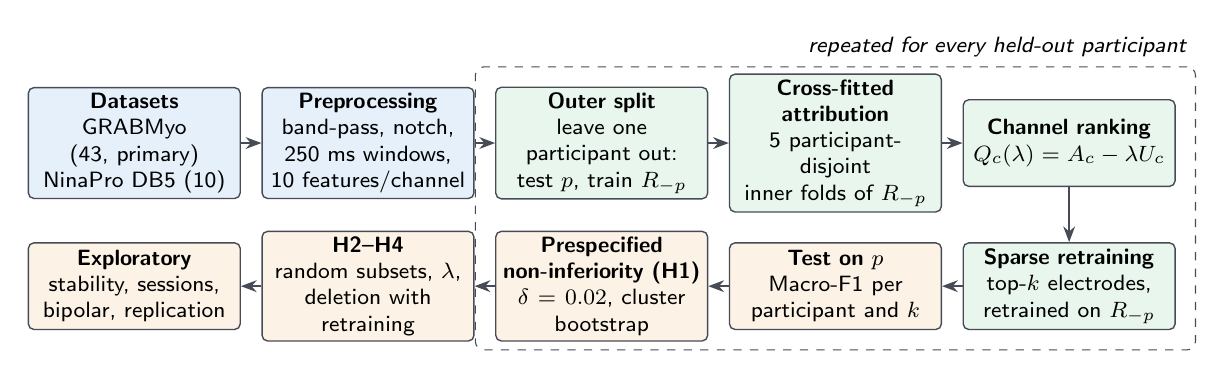
\begin{tikzpicture}[
  font=\footnotesize,
  box/.style={draw=edgeC, rounded corners=2pt, align=center, text width=25.5mm, execute at begin node={\hyphenpenalty=10000\relax},
              minimum height=11mm, inner sep=2pt, line width=0.5pt},
  arr/.style={-{Stealth[length=2mm]}, line width=0.6pt, draw=edgeC},
  node distance=4mm and 2.6mm]
% row 1: data to ranking
\node[box, fill=dataC] (data) {\textbf{Datasets}\\GRABMyo (43, primary)\\NinaPro DB5 (10)};
\node[box, fill=dataC, right=of data] (pre) {\textbf{Preprocessing}\\band-pass, notch,\\250 ms windows,\\10 features/channel};
\node[box, fill=loopC, right=of pre] (outer) {\textbf{Outer split}\\leave one participant out:\\test $p$, train $R_{-p}$};
\node[box, fill=loopC, right=of outer] (inner) {\textbf{Cross-fitted attribution}\\5 participant-disjoint\\inner folds of $R_{-p}$};
\node[box, fill=loopC, right=of inner] (rank) {\textbf{Channel ranking}\\$Q_c(\lambda) = A_c - \lambda U_c$};
% row 2: retraining and evaluation
\node[box, fill=loopC, below=7mm of rank] (sparse) {\textbf{Sparse retraining}\\top-$k$ electrodes,\\retrained on $R_{-p}$};
\node[box, fill=testC, left=of sparse] (test) {\textbf{Test on $p$}\\Macro-F1 per\\participant and $k$};
\node[box, fill=testC, left=of test] (ni) {\textbf{Prespecified}\\\textbf{non-inferiority (H1)}\\$\delta = 0.02$, cluster bootstrap};
\node[box, fill=testC, left=of ni] (h24) {\textbf{H2--H4}\\random subsets, $\lambda$,\\deletion with retraining};
\node[box, fill=testC, left=of h24] (expl) {\textbf{Exploratory}\\stability, sessions,\\bipolar, replication};
\draw[arr] (data) -- (pre);
\draw[arr] (pre) -- (outer);
\draw[arr] (outer) -- (inner);
\draw[arr] (inner) -- (rank);
\draw[arr] (rank) -- (sparse);
\draw[arr] (sparse) -- (test);
\draw[arr] (test) -- (ni);
\draw[arr] (ni) -- (h24);
\draw[arr] (h24) -- (expl);
\begin{scope}[on background layer]
  \node[draw=edgeC, dashed, rounded corners=3pt, inner sep=2.5mm, fit=(outer)(rank)(sparse)(test),
        label={[font=\footnotesize\itshape, anchor=south east]north east:repeated for every held-out participant}] {};
\end{scope}
\end{tikzpicture}
\end{document}
